\documentclass[12pt,a4paper]{article}
% The following LaTeX packages must be installed on your machine: amsmath, authblk, bm, booktabs, caption, dcolumn, fancyhdr, geometry, graphicx, hyperref, latexsym, natbib
\input{183.dat}
\usepackage{gensymb}
\usepackage{amsthm}
\usepackage{float}
\usepackage{siunitx}
\usepackage{amssymb}
\usepackage{float}
\usepackage{enumerate}
\usepackage{listings}
\usepackage{mathtools}
\PassOptionsToPackage{hyphens}{url}\usepackage{hyperref}
\usepackage[none]{hyphenat}
\usepackage{physics}
%\renewcommand{\familydefault}{\sfdefault}


\begin{document}

\setcounter{page}{1}

\section*{Bode Plots}
\bigskip

\begin{figure}[!h]
	\centering
	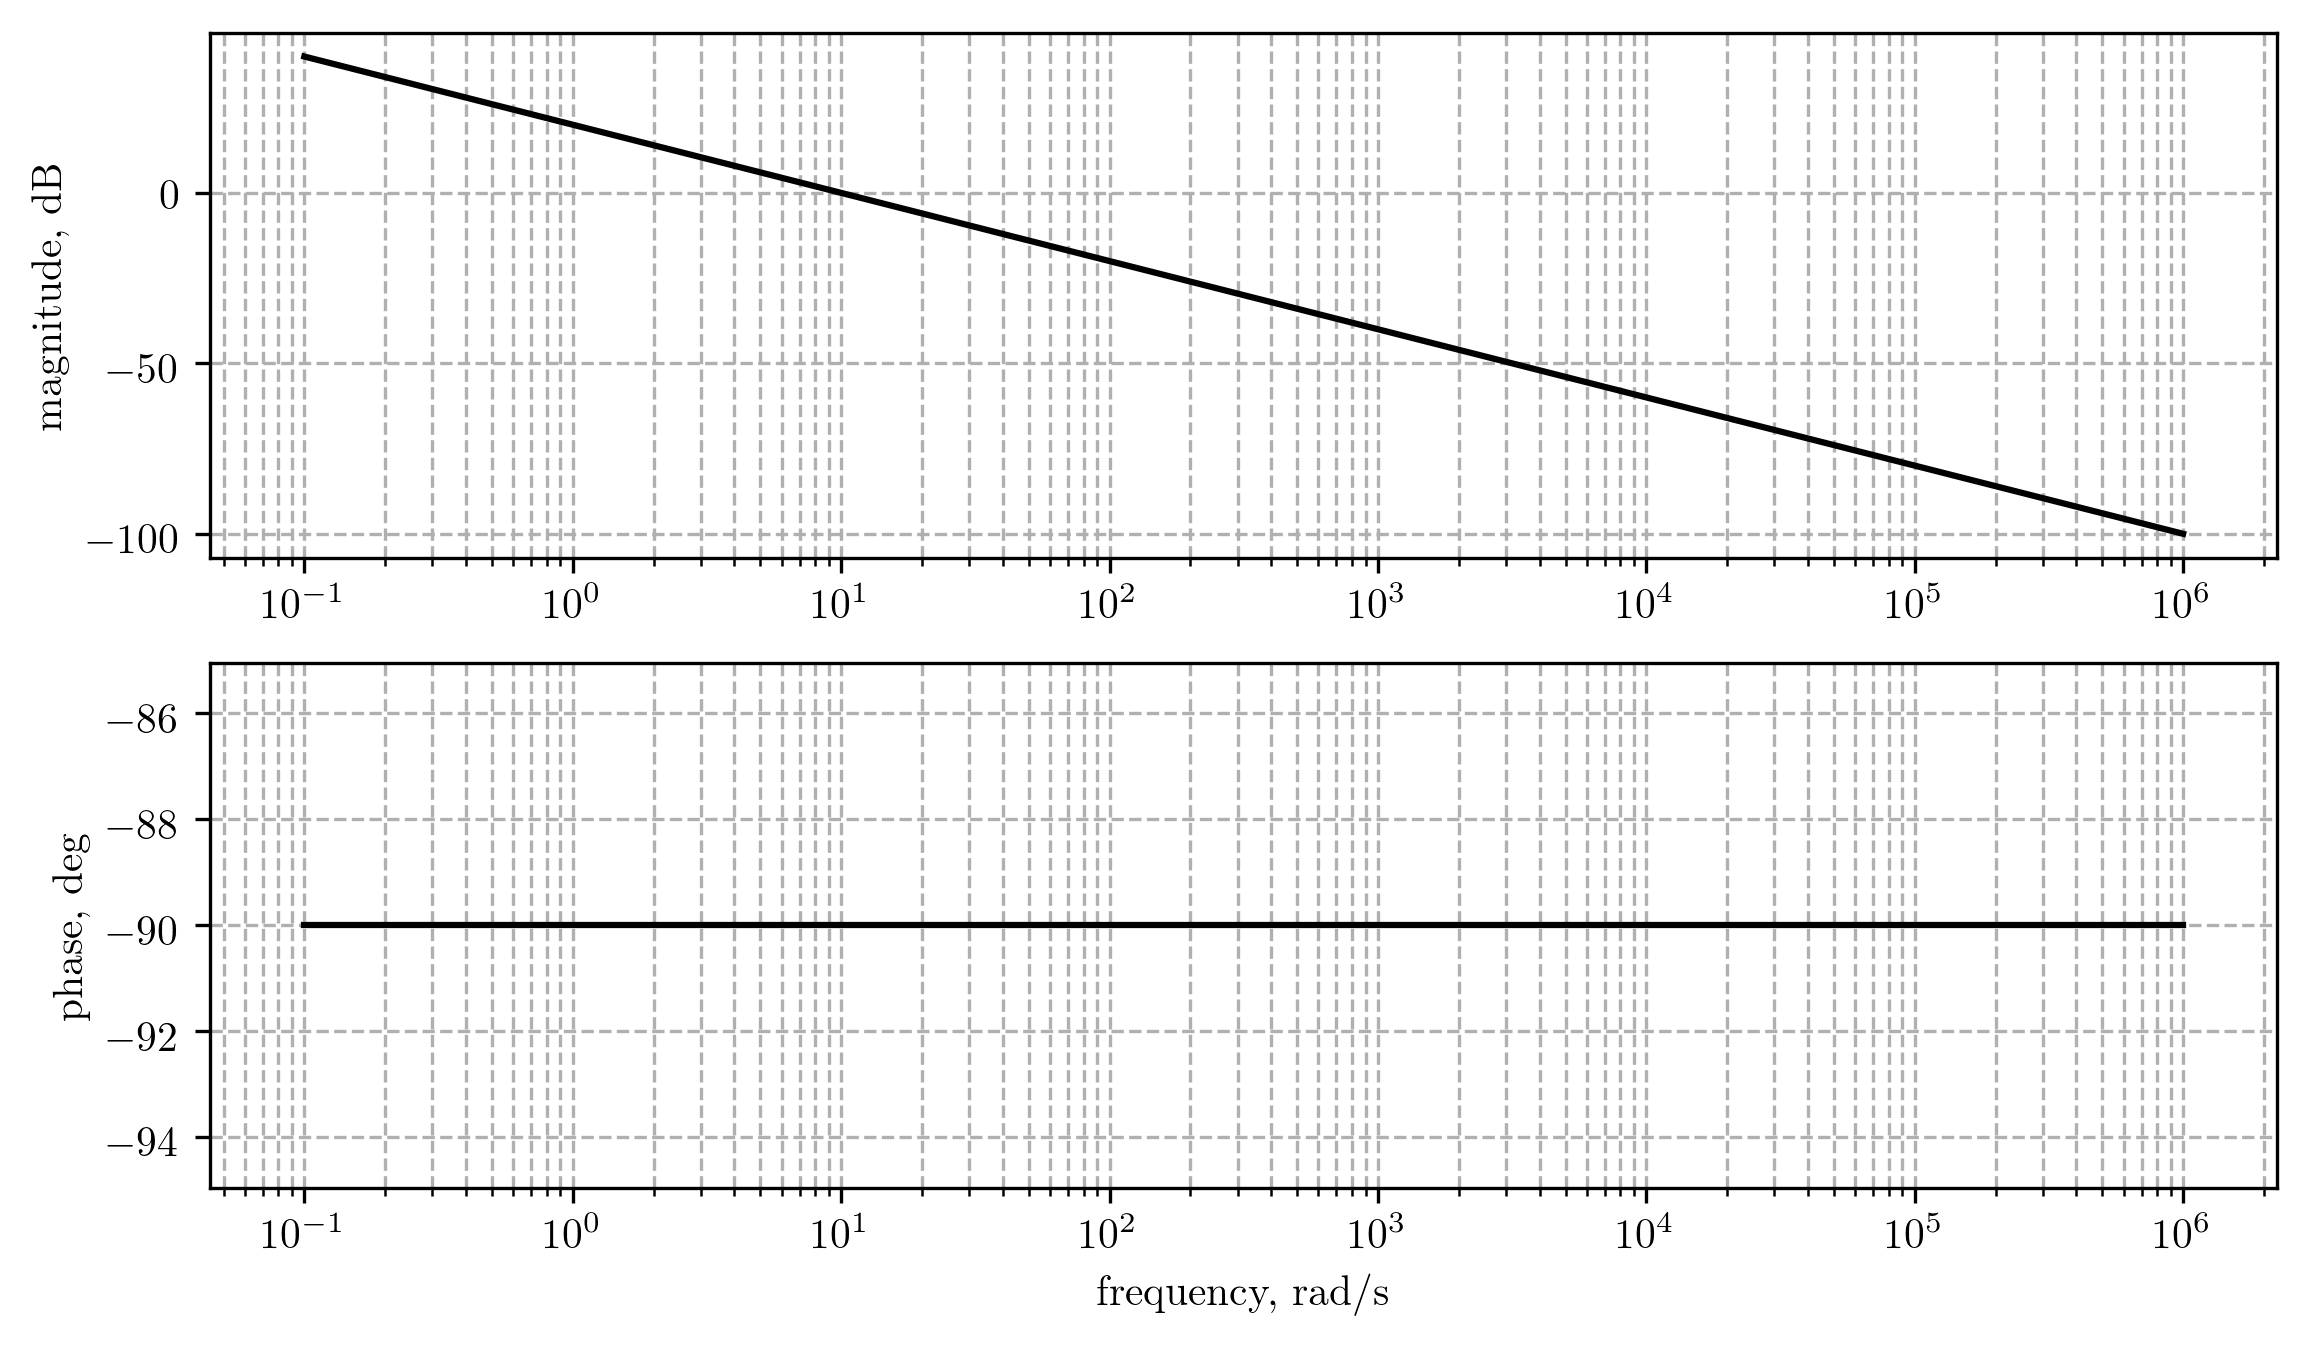
\includegraphics[width=\linewidth]{0.png}
	\caption{Bode plot for $G(s) = \frac{10}{s}$. My manual estimate is the same as the actual plot.}
\end{figure}

\begin{figure}[!h]
	\centering
	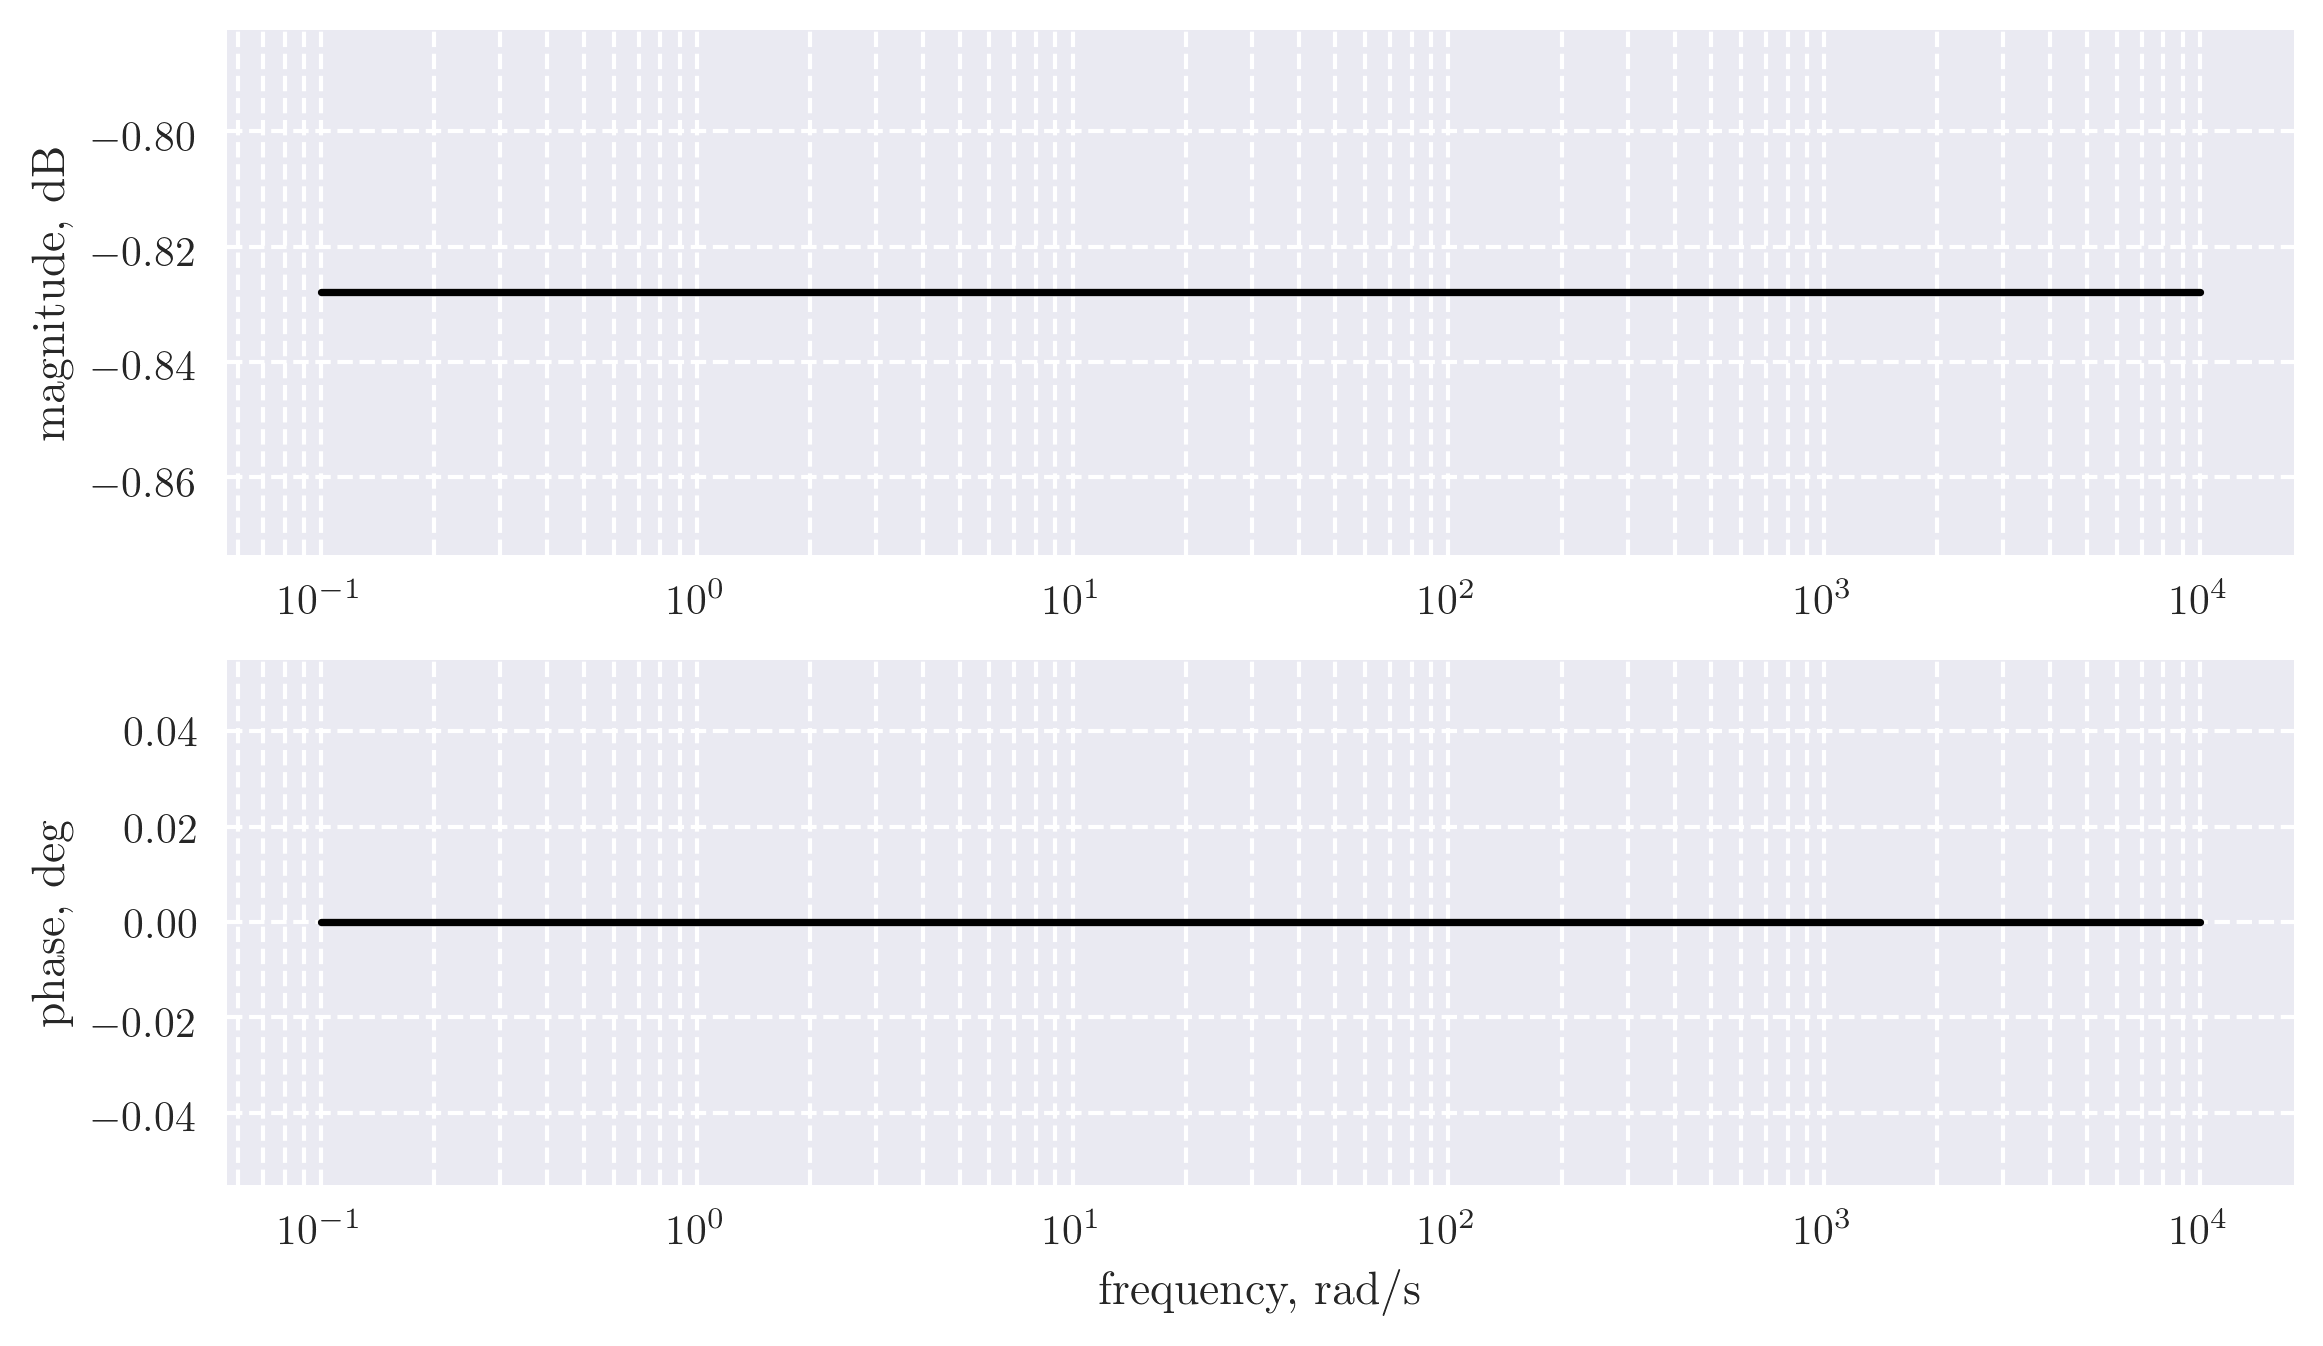
\includegraphics[width=\linewidth]{1.png}
	\caption{Bode plot for $G(s) = 10s$. My manual estimate for the phase plot is correct. However, my estimate for the magnitude plot is incorrect (it should have a positive slope).}
\end{figure}

\begin{figure}[!h]
	\centering
	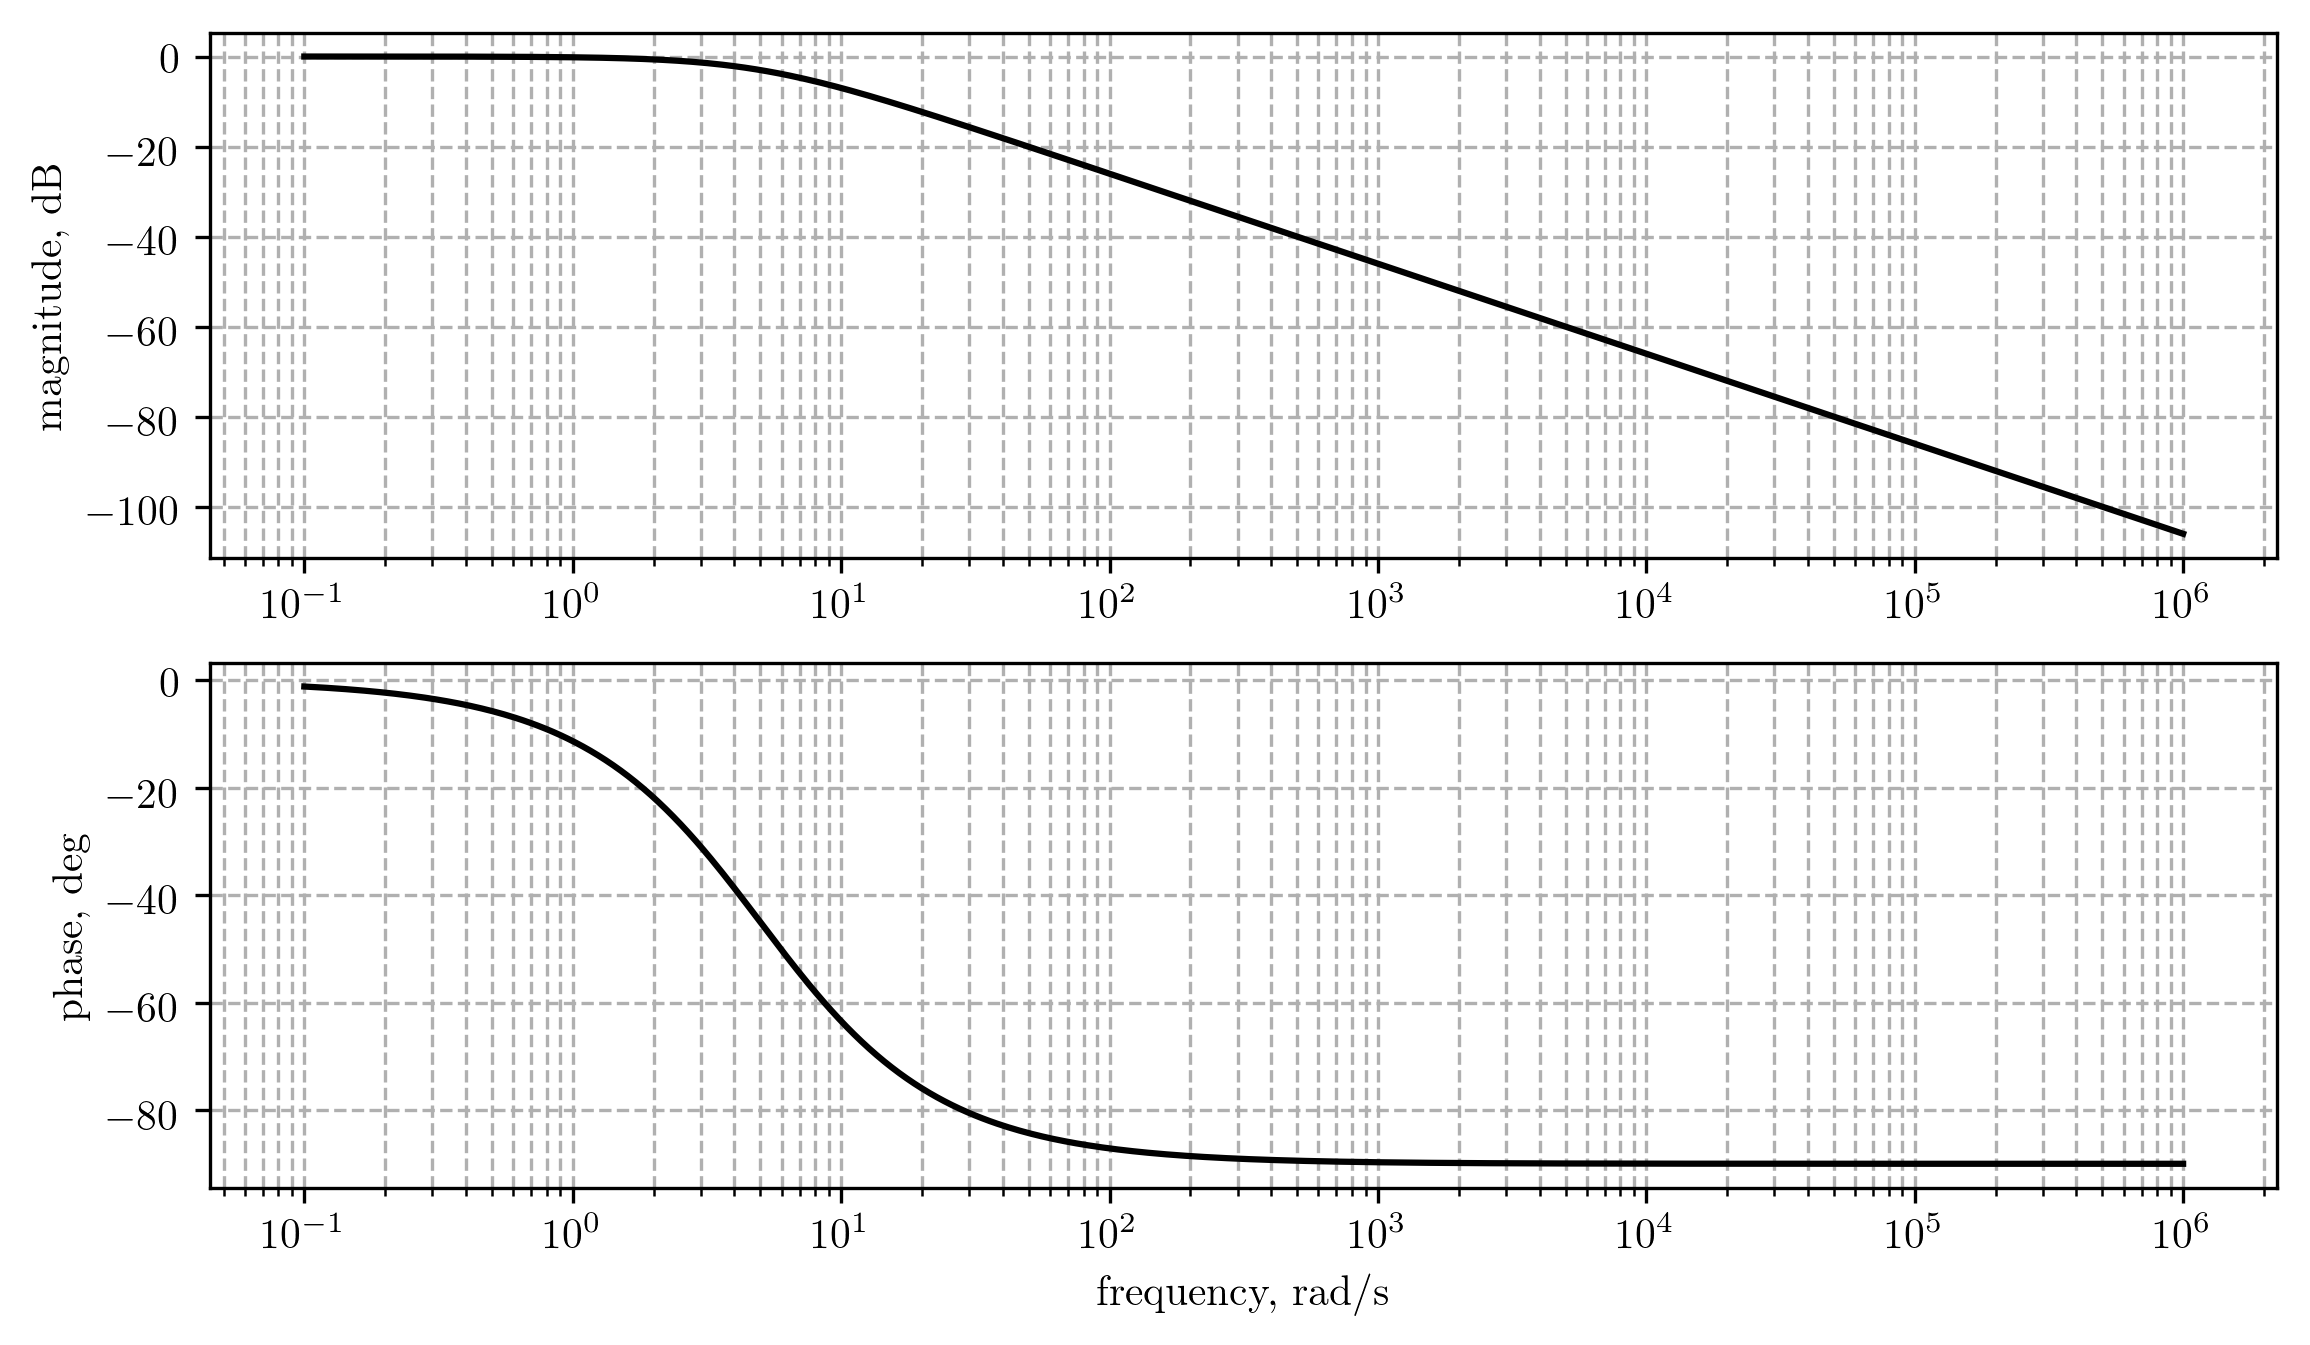
\includegraphics[width=\linewidth]{2.png}
	\caption{Bode plot for $G(s) = \frac{5}{s+5}$. My manual estimate is the same as the actual plot.}
\end{figure}

\begin{figure}[!h]
	\centering
	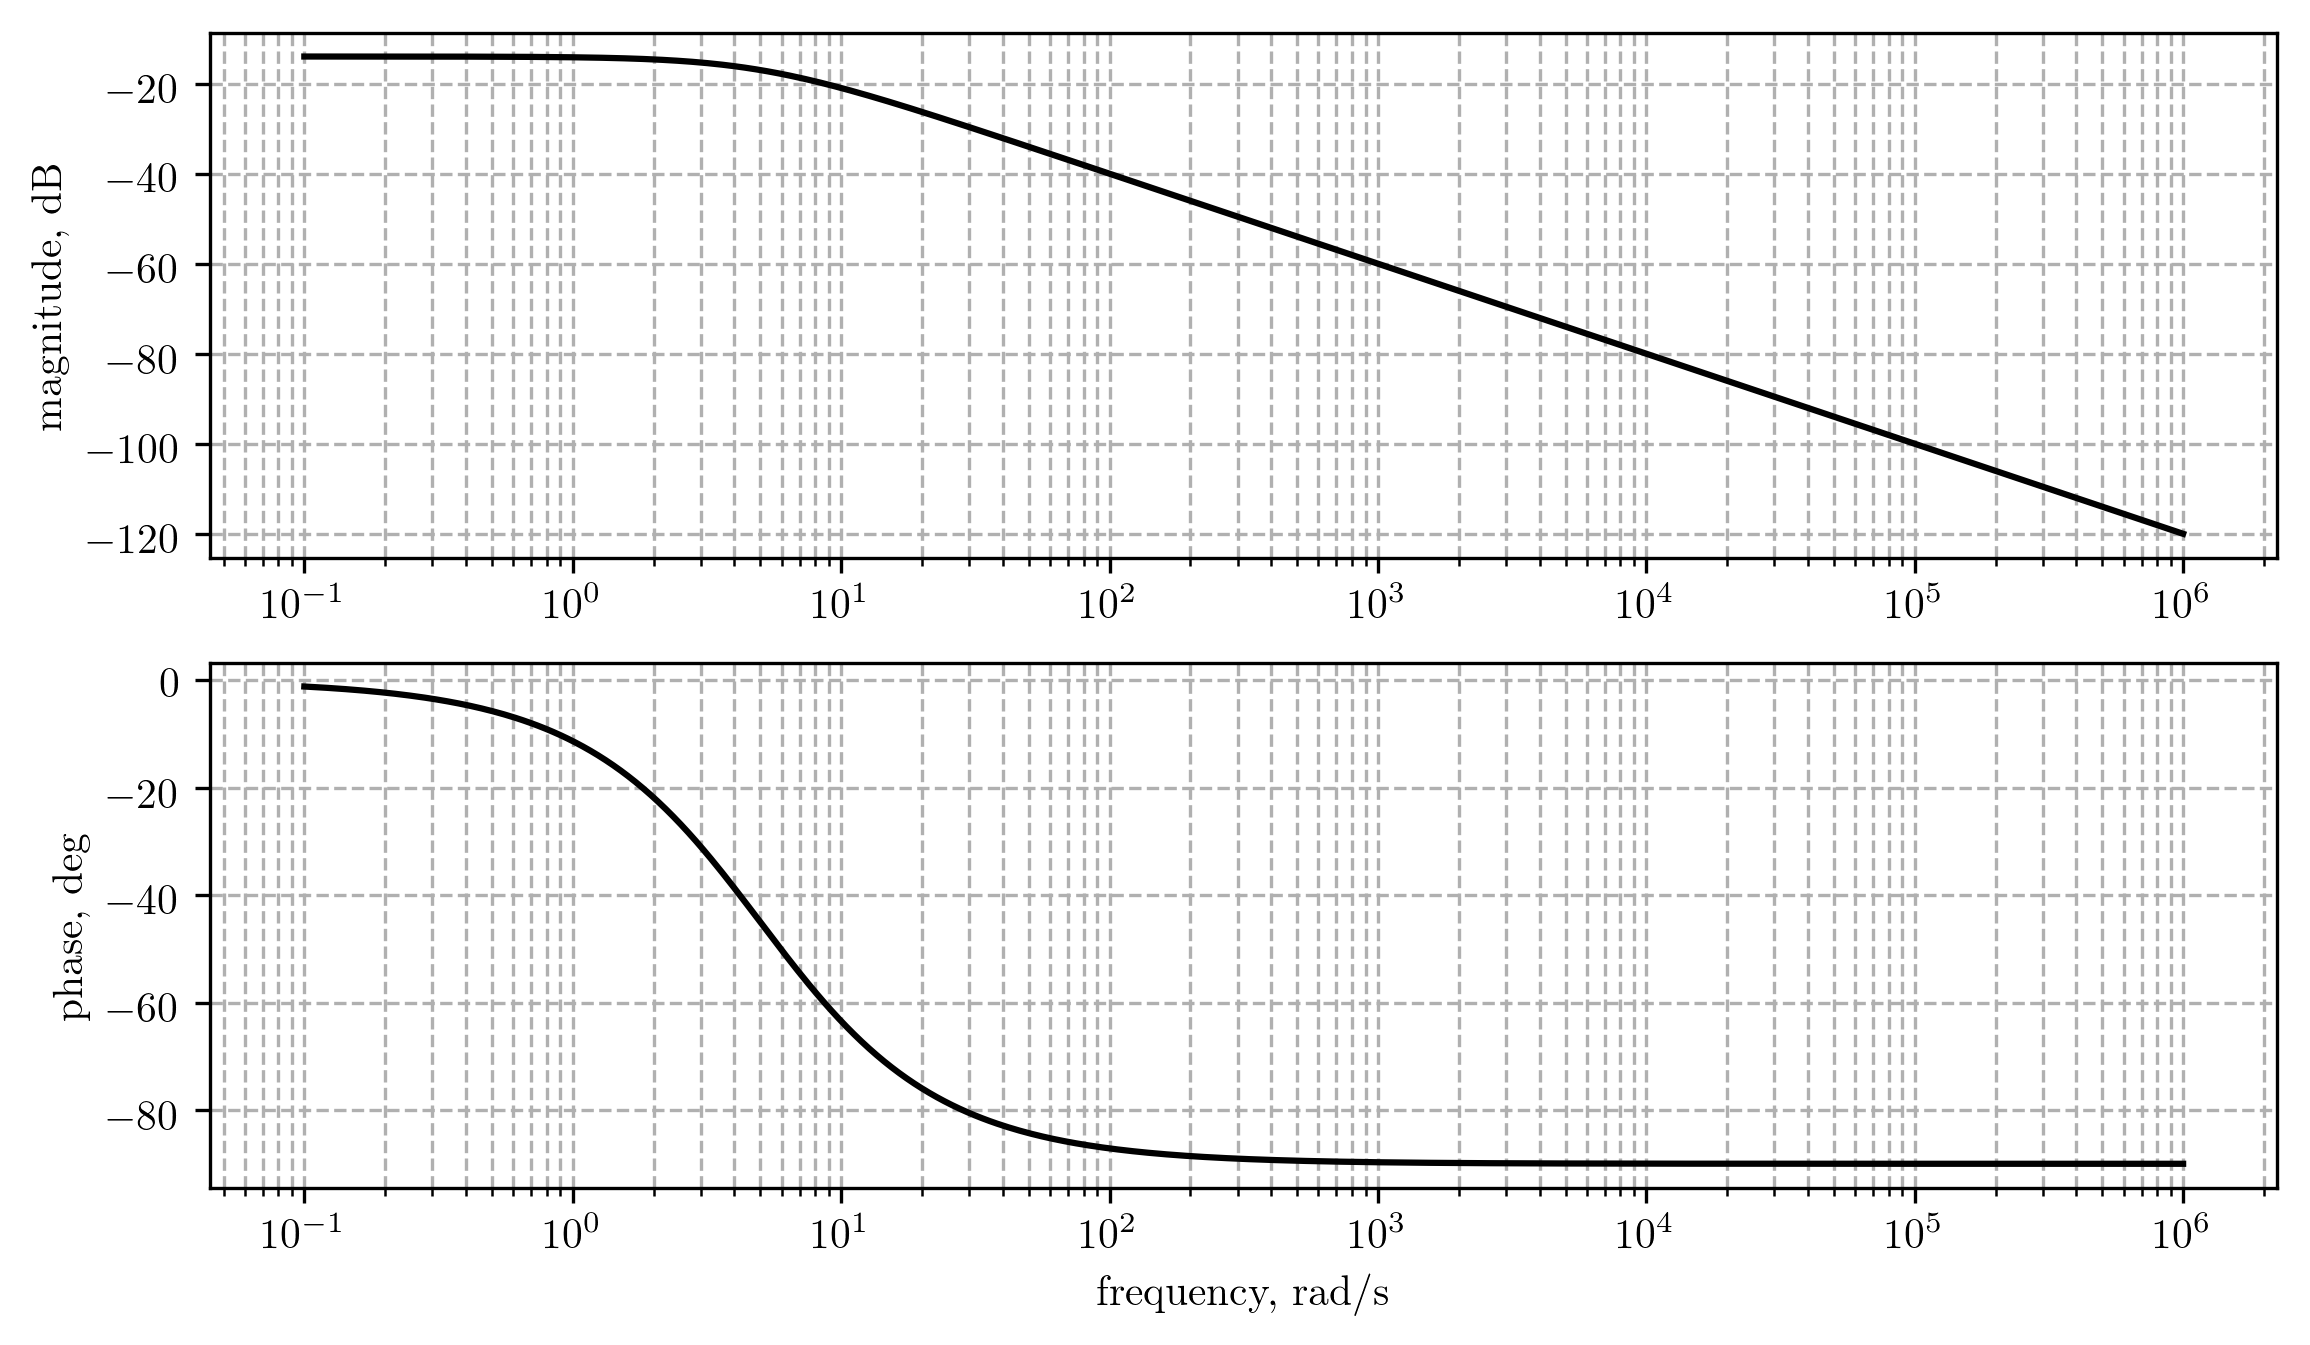
\includegraphics[width=\linewidth]{3.png}
	\caption{Bode plot for $G(s) = \frac{1}{s+5}$. My manual estimate is the same as the actual plot.}
\end{figure}

\begin{figure}[!h]
	\centering
	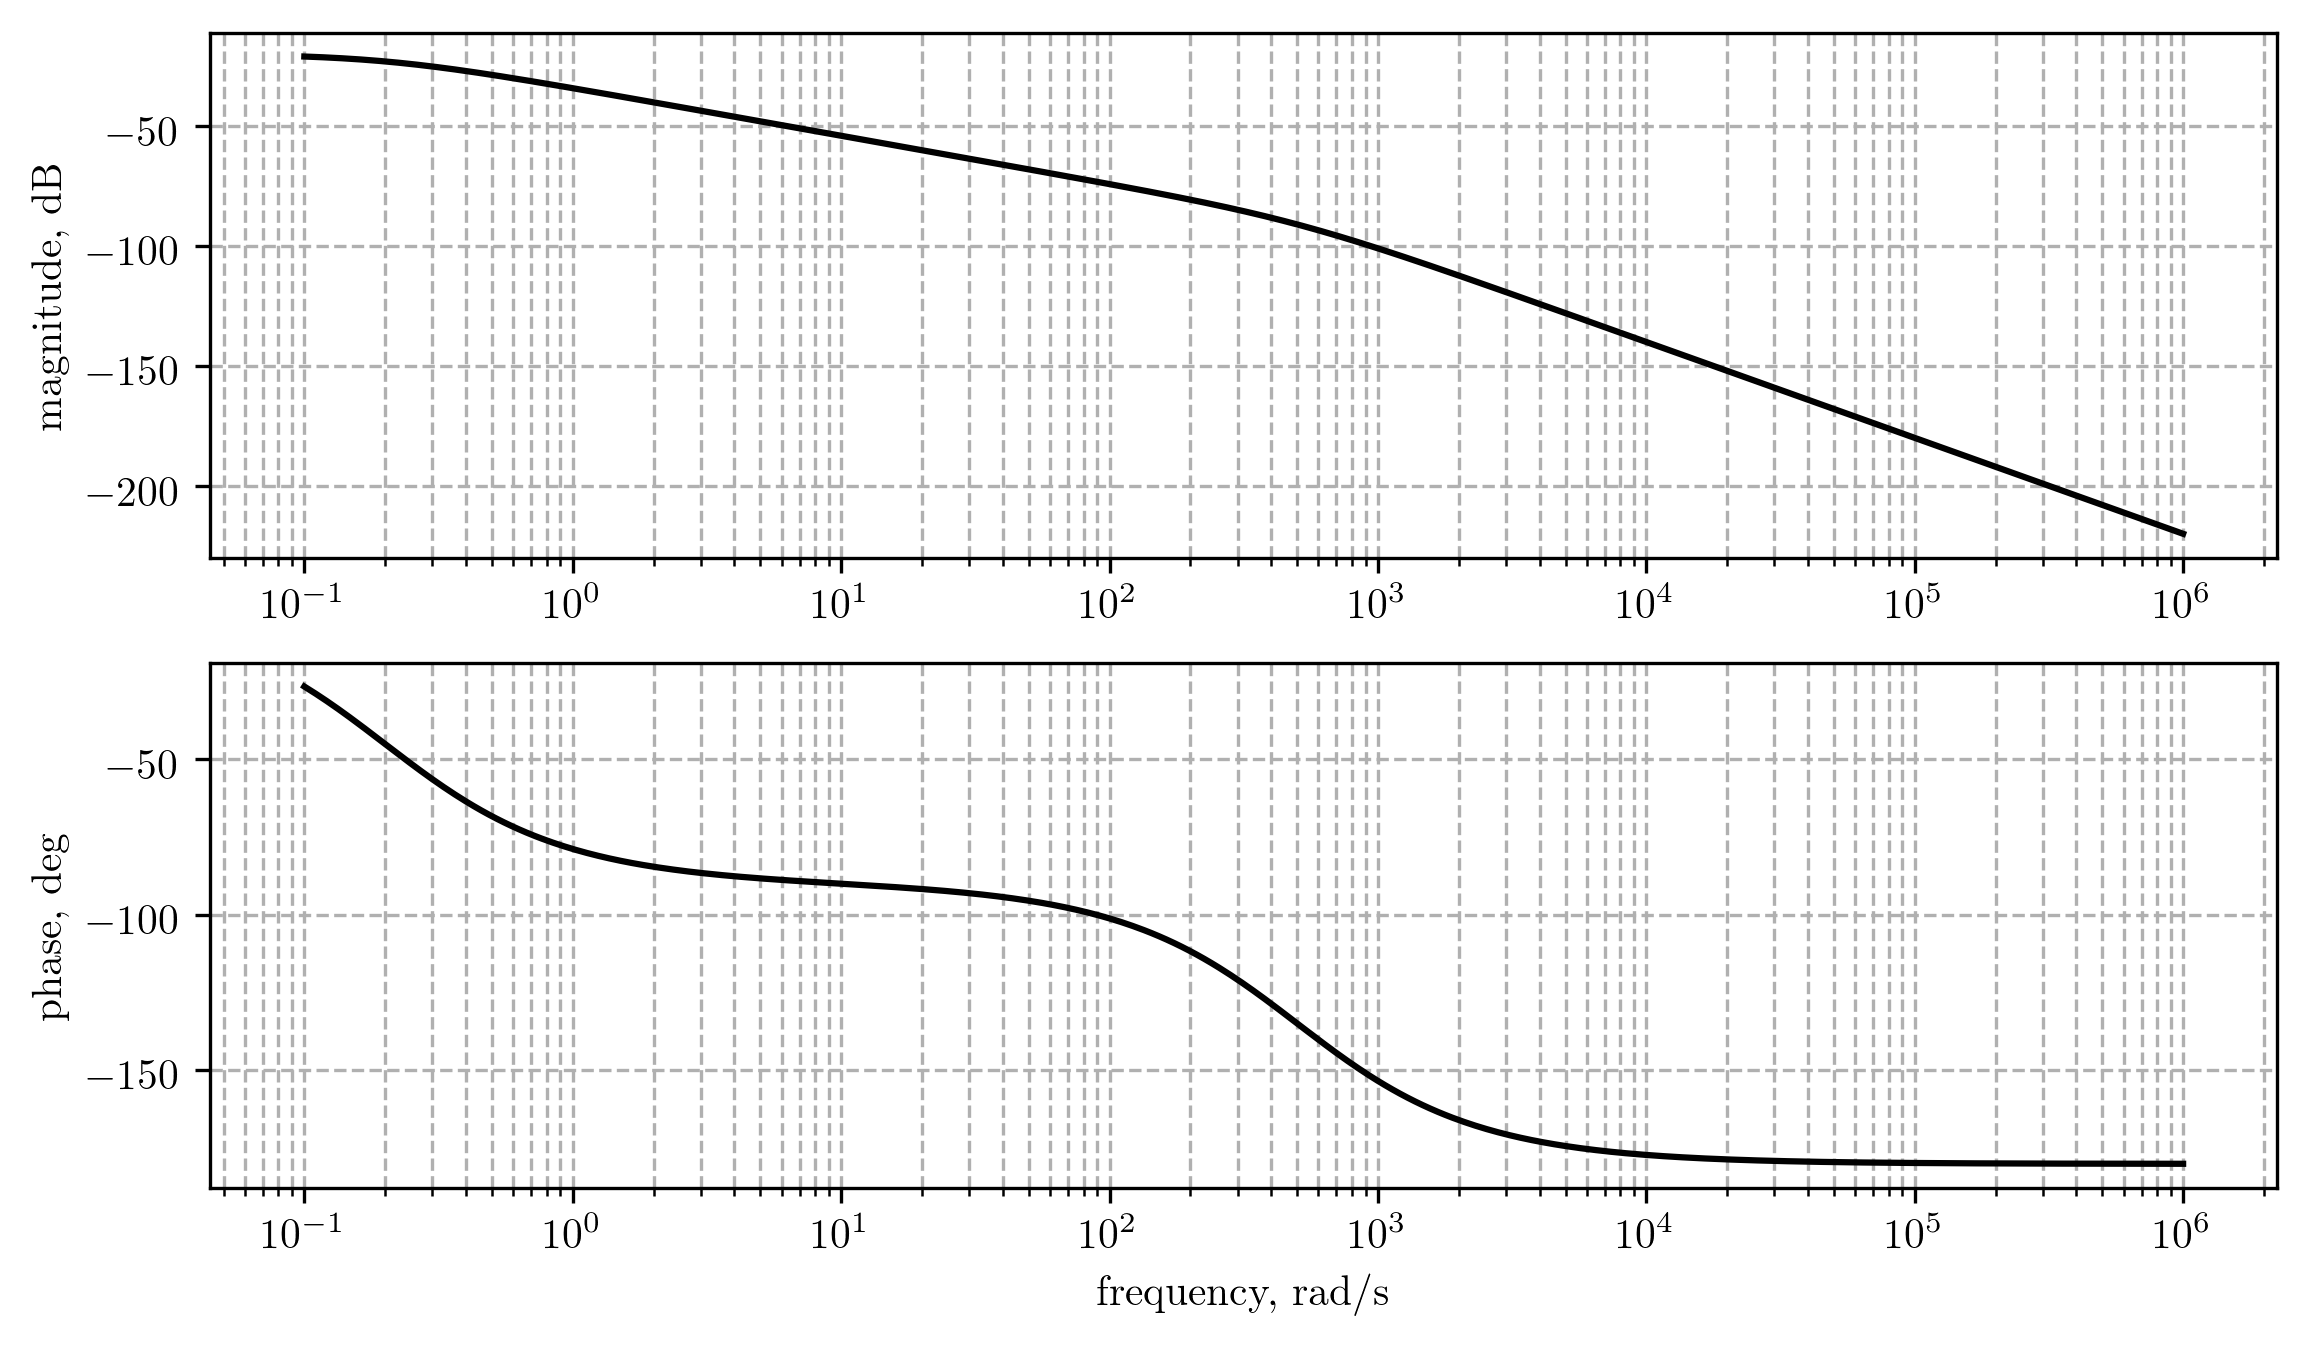
\includegraphics[width=\linewidth]{4.png}
	\caption{Bode plot for $G(s) = \frac{10}{(s+2)(s+500)}$. My manual estimate is the same as the actual plot.}
\end{figure}

\begin{figure}[!h]
	\centering
	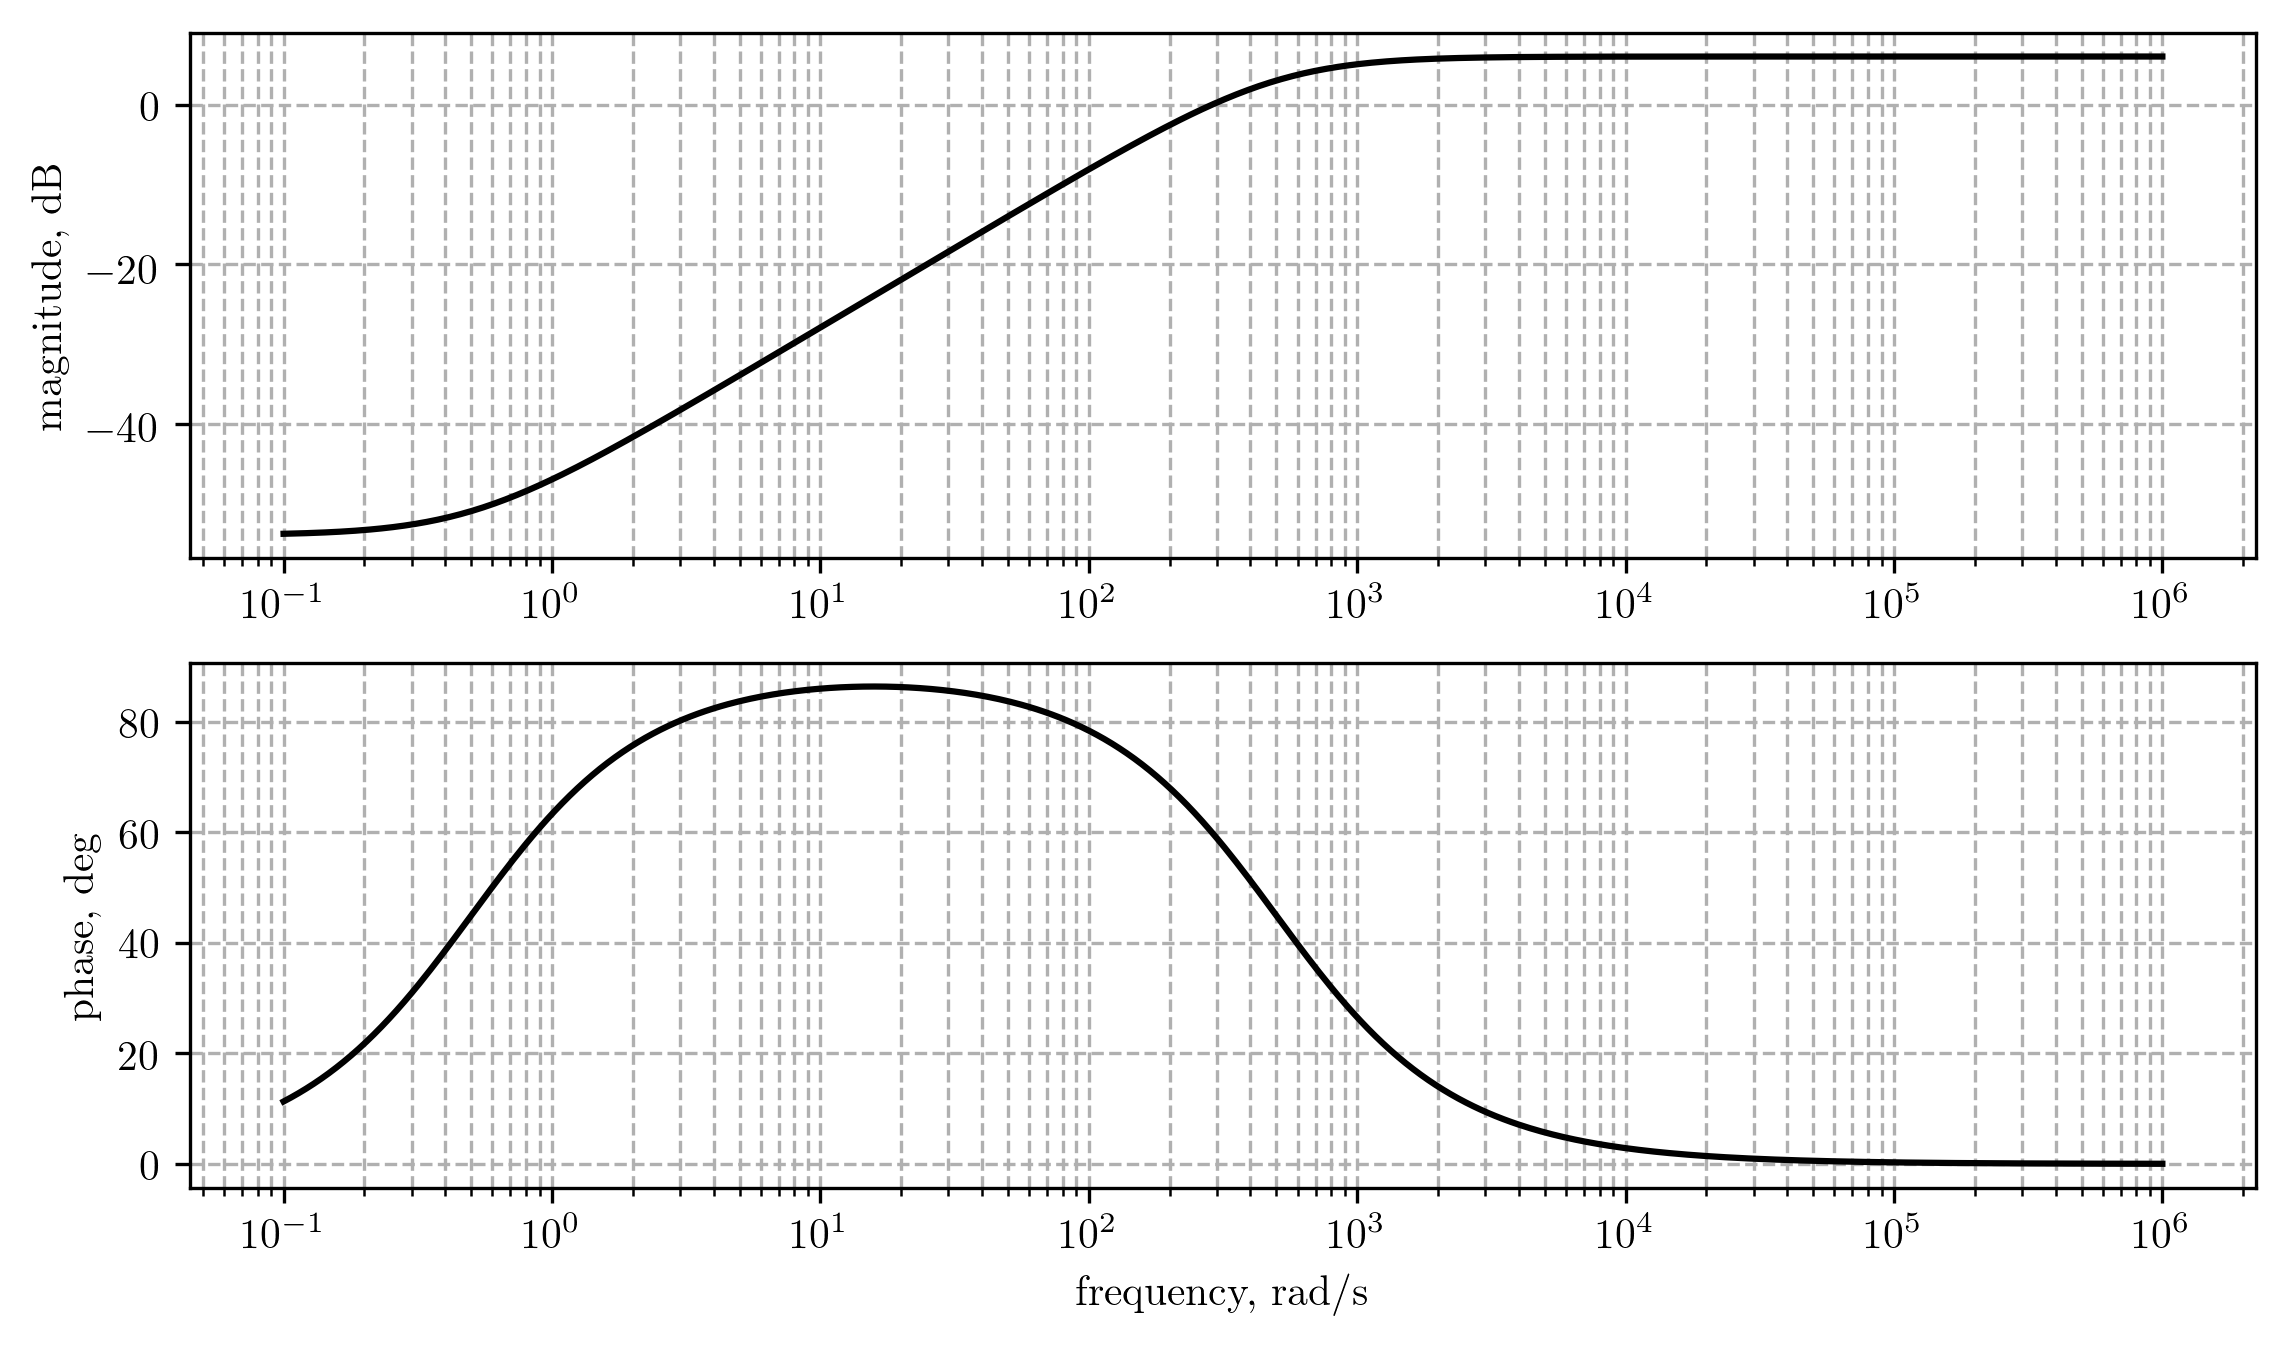
\includegraphics[width=\linewidth]{5.png}
	\caption{Bode plot for $G(s) = \frac{s+2}{s+500}$. My manual estimate is the same as the actual plot.}
\end{figure}

\begin{figure}[!h]
	\centering
	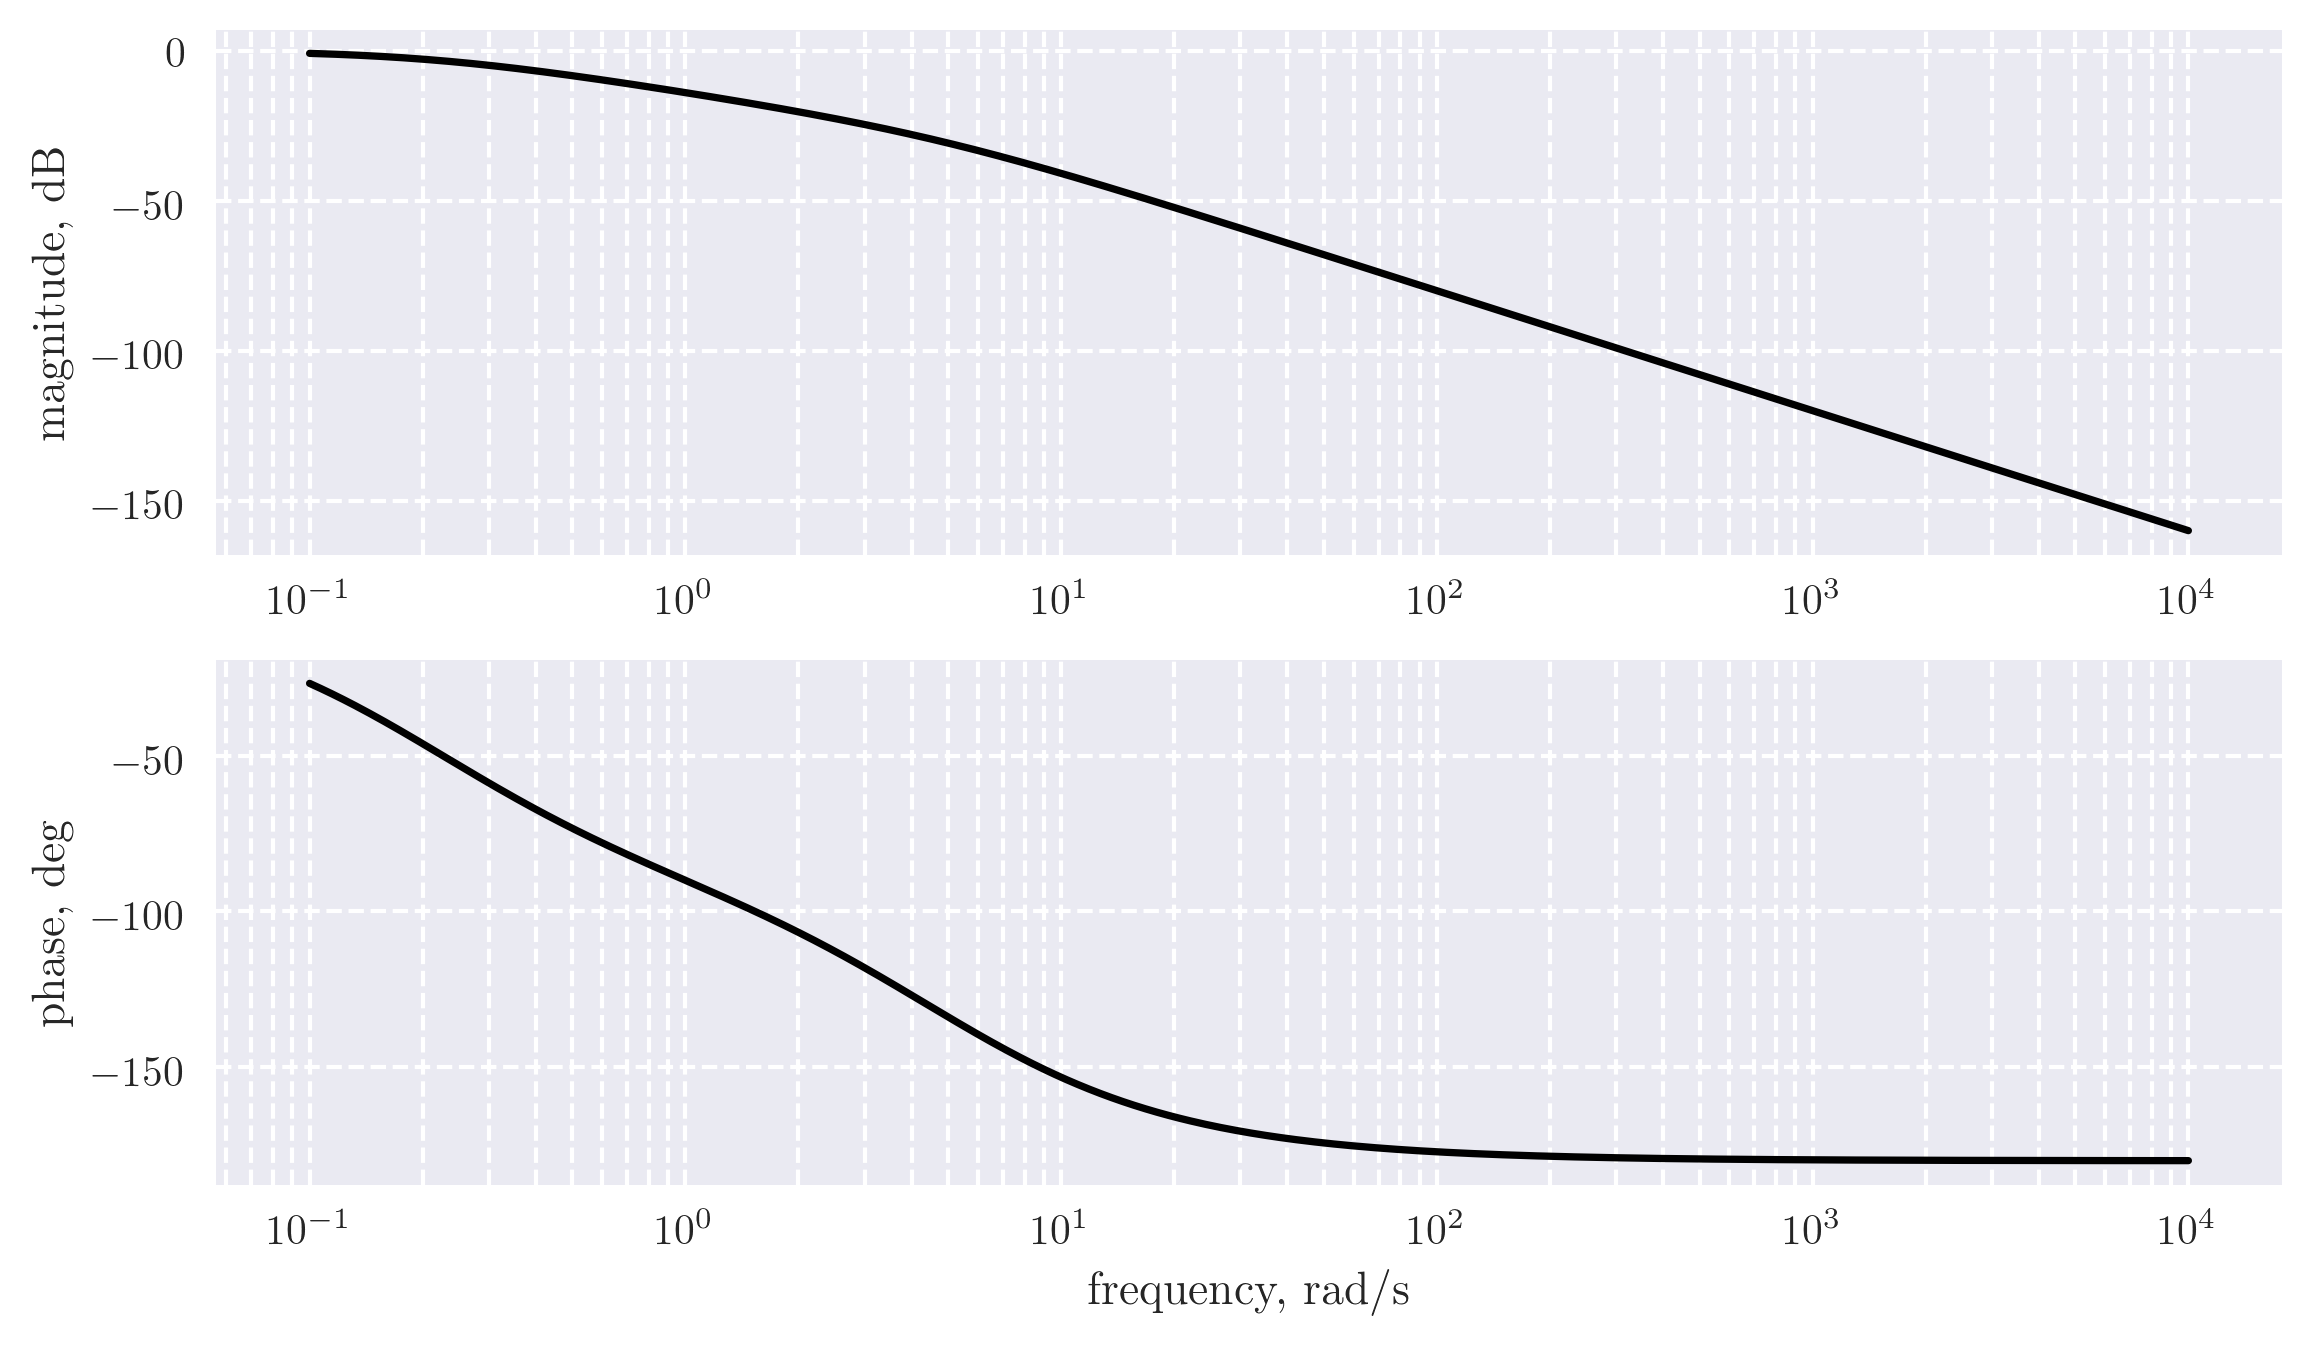
\includegraphics[width=\linewidth]{6.png}
	\caption{Bode plot for $G(s) = \frac{1}{s(s+5)}$. My manual estimate is the same as the actual plot.}
\end{figure}

\begin{figure}[!h]
	\centering
	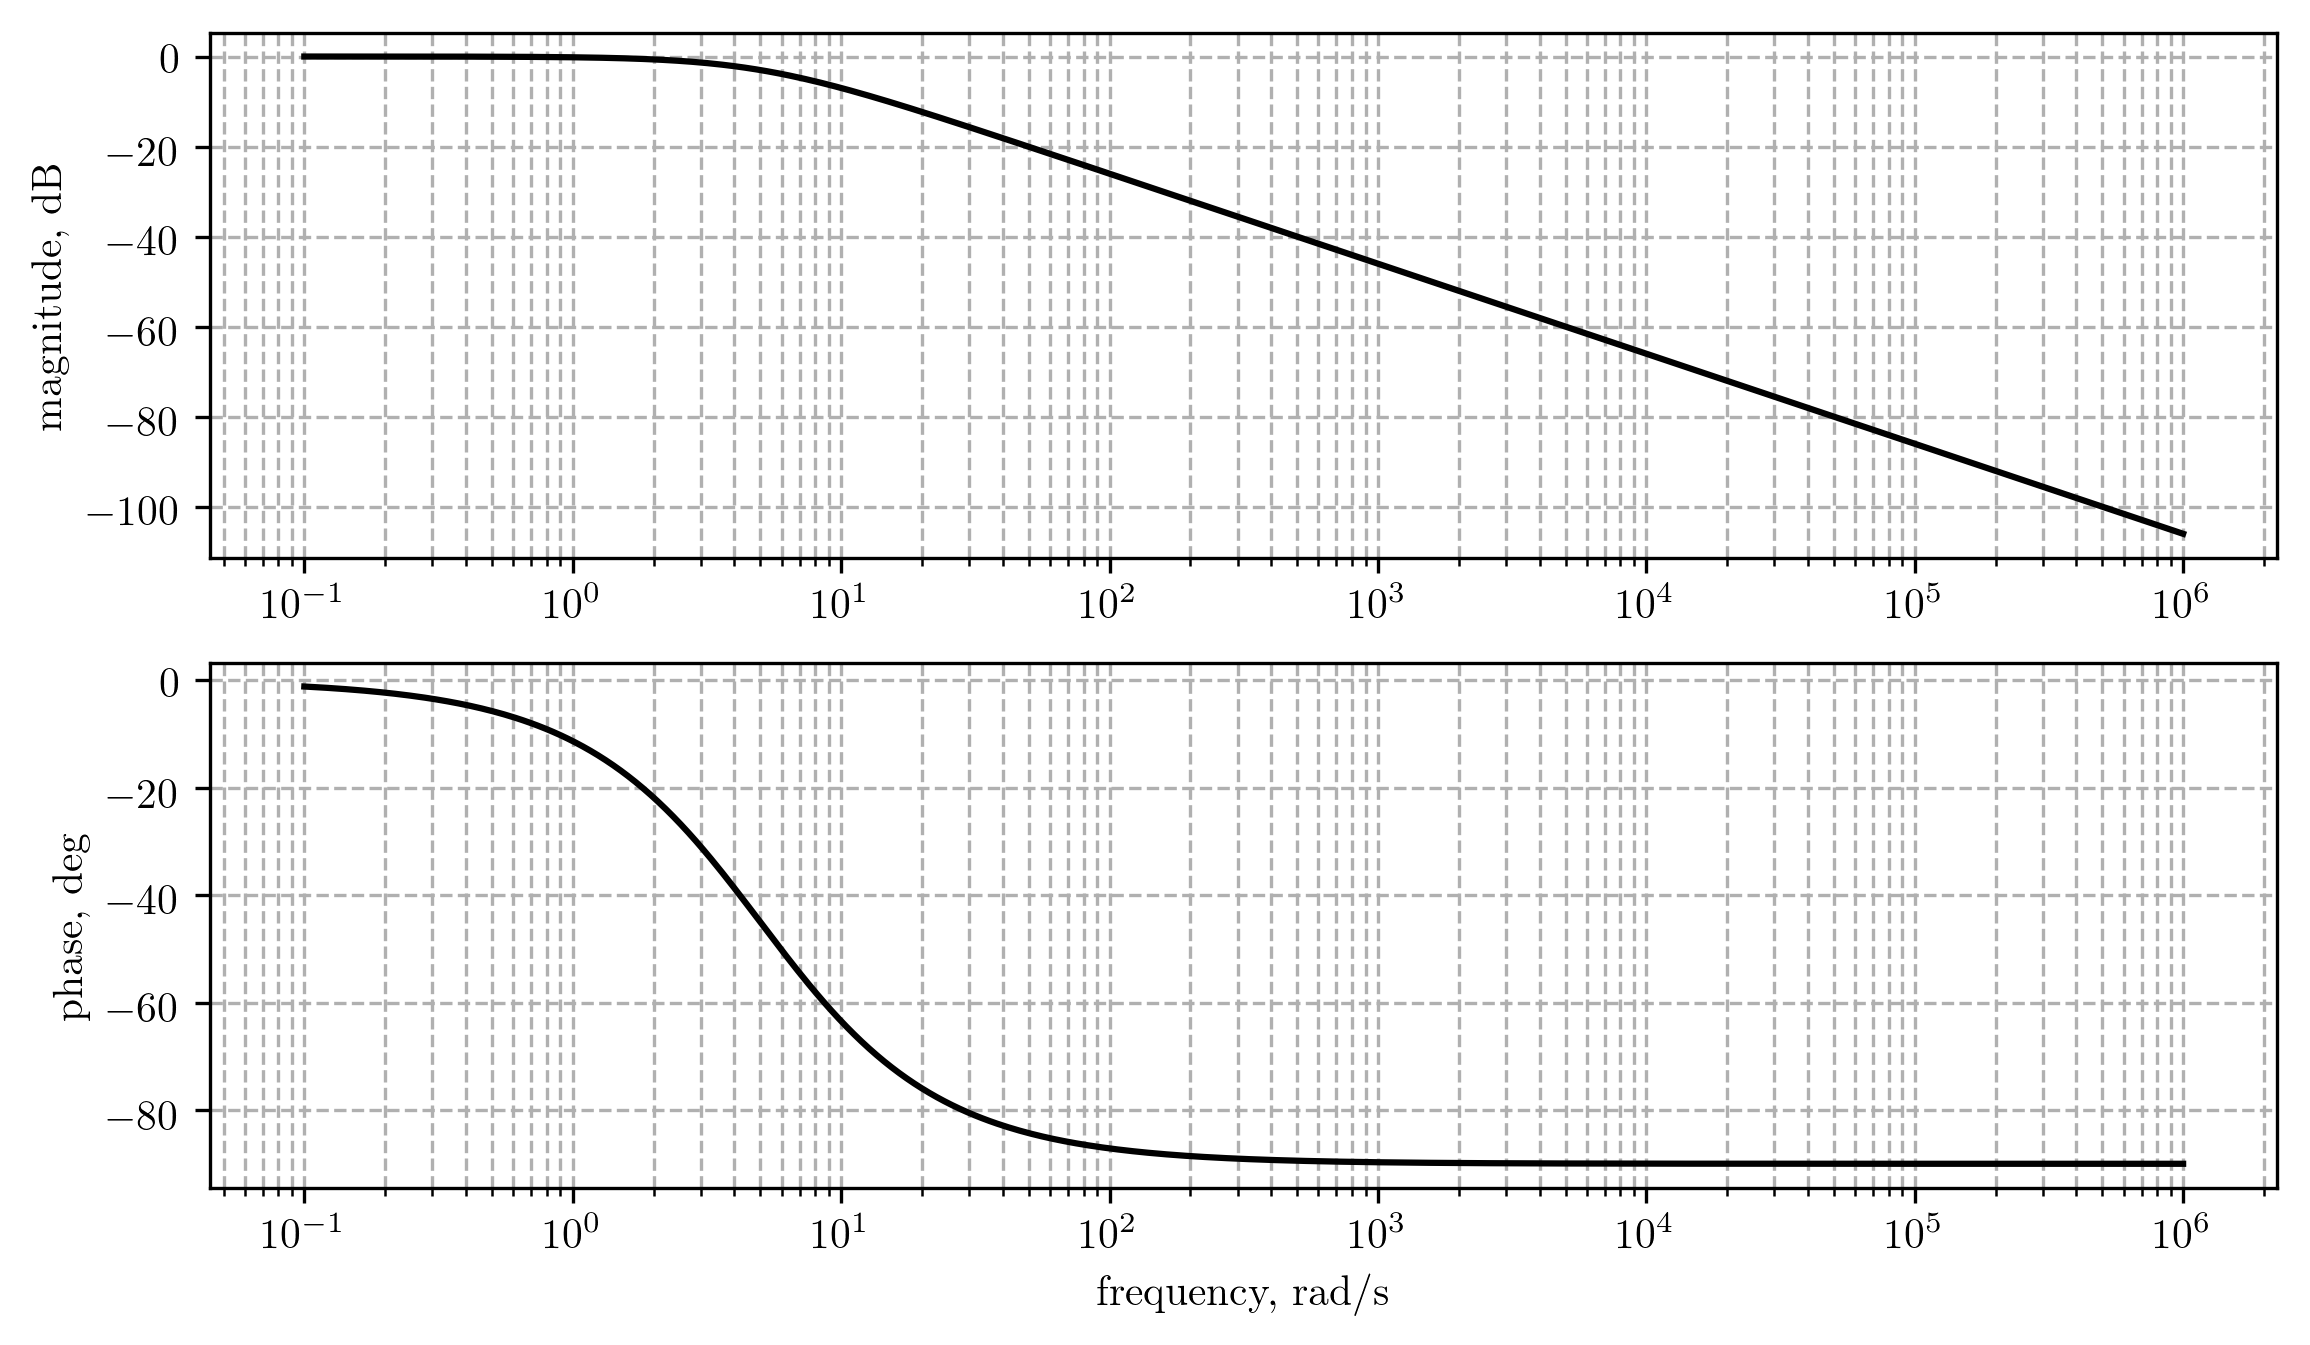
\includegraphics[width=\linewidth]{7.png}
	\caption{Bode plot for $G(s) = \frac{5s}{s+5}$. My manual estimate is the same as the actual plot.}
\end{figure}

\begin{figure}[!h]
	\centering
	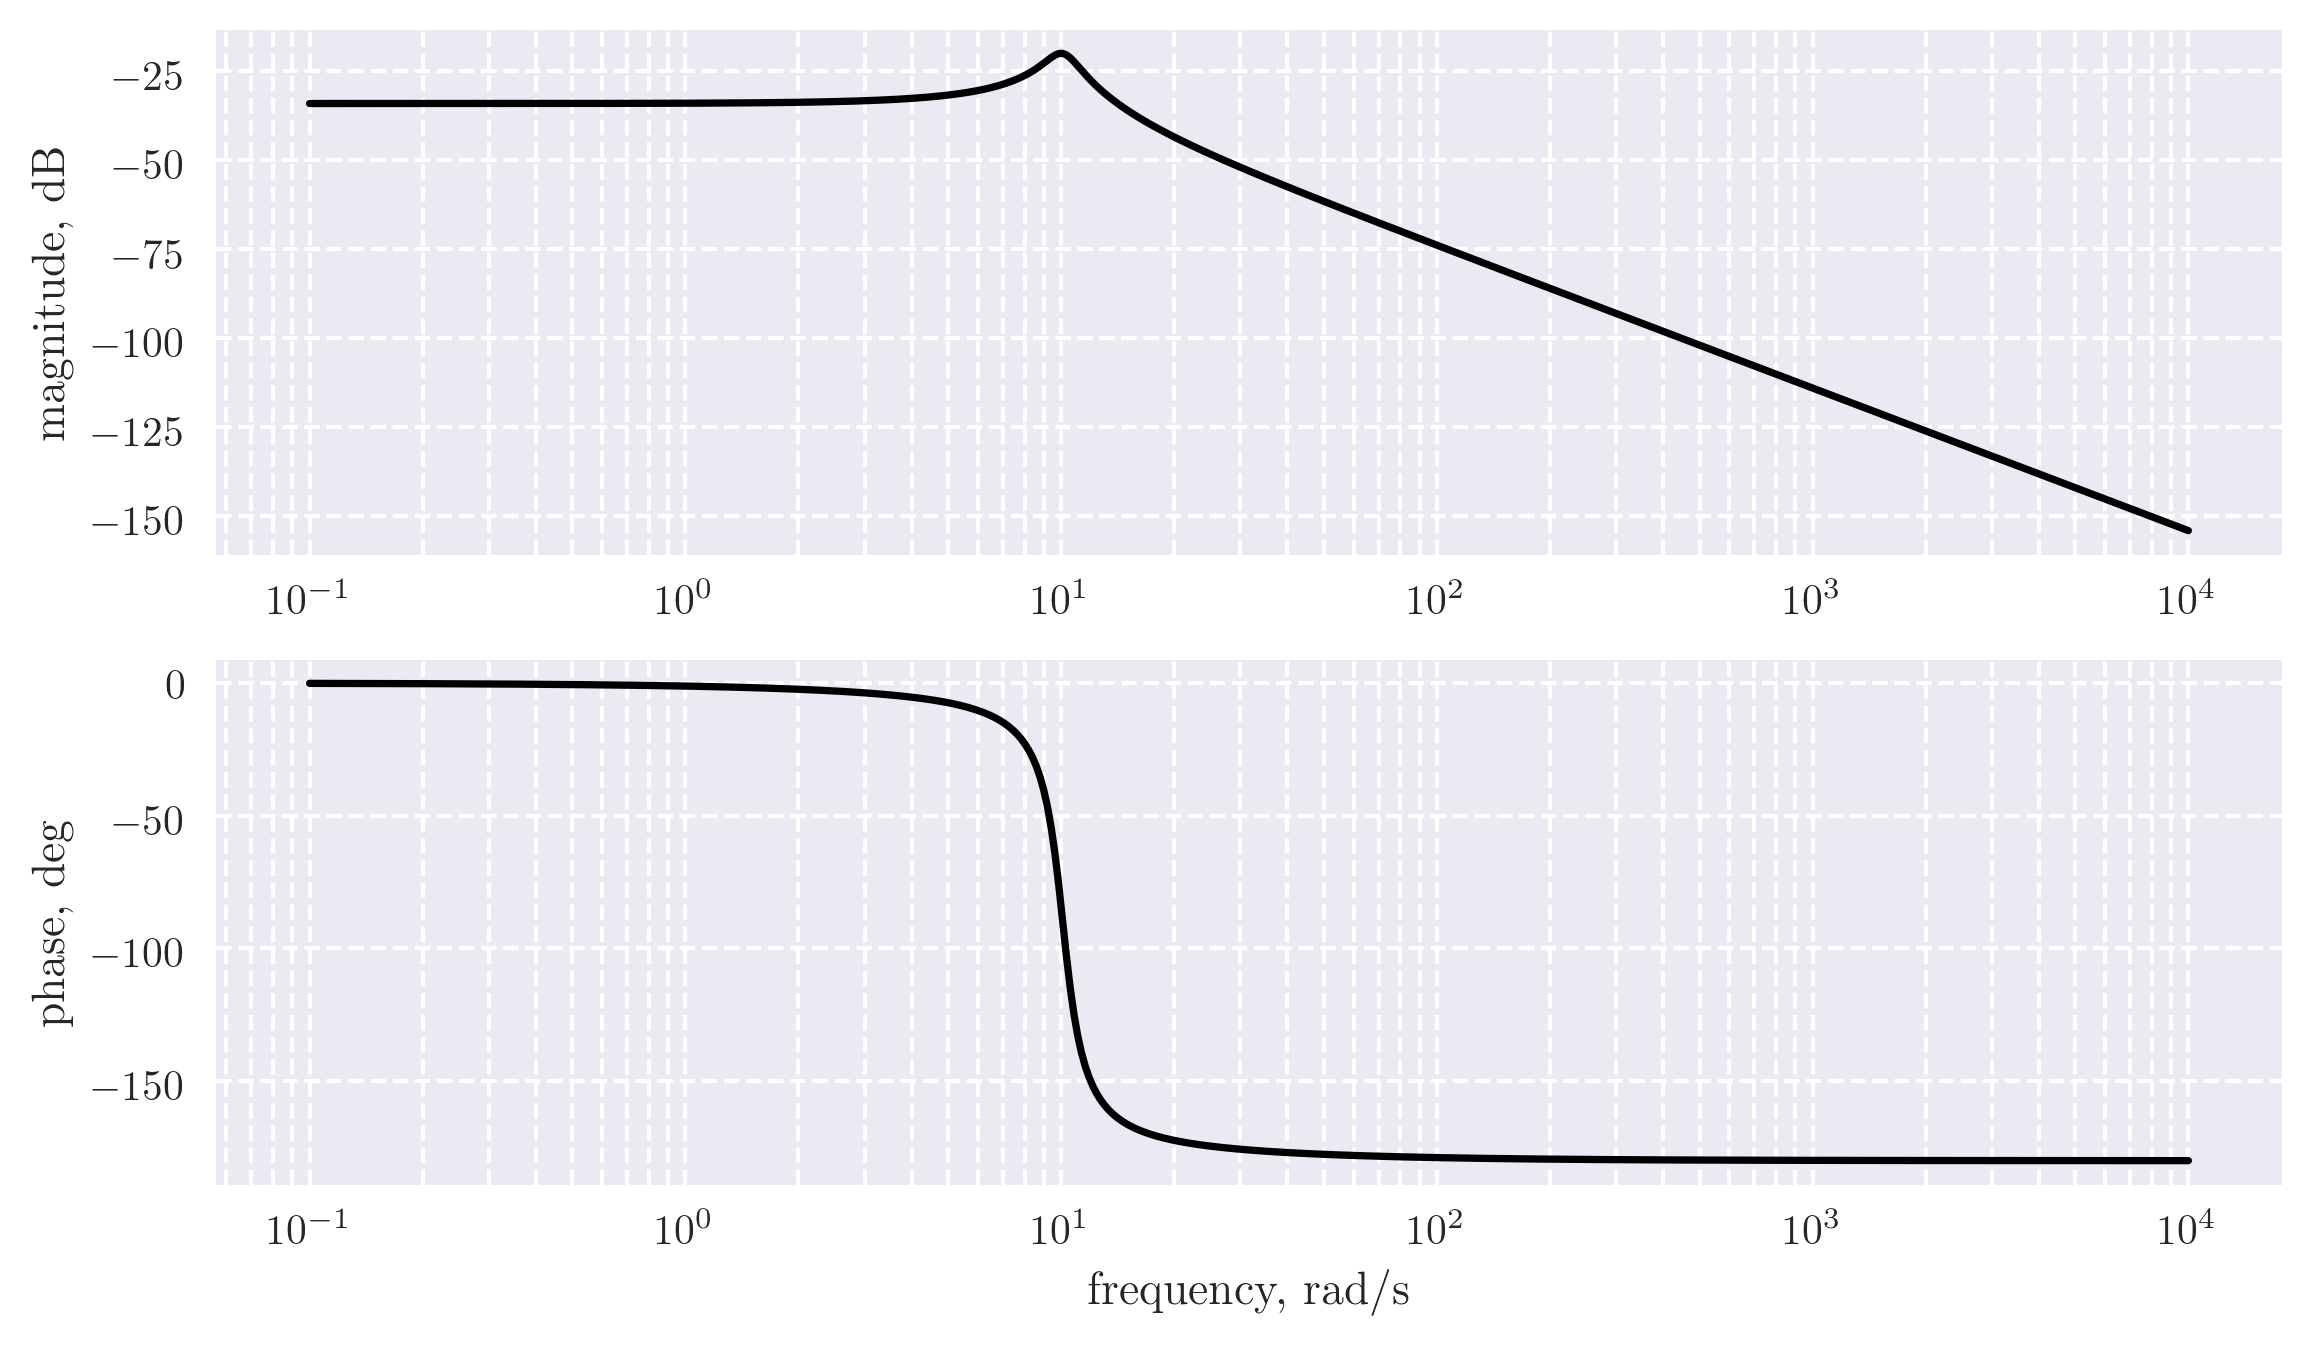
\includegraphics[width=\linewidth]{8.png}
	\caption{Bode plot for $G(s) = \frac{2}{s^2+2s+100}$. My manual estimate is the same as the actual plot.}
\end{figure}

\end{document}